\chapter{Introduction} 
\label{ch:introduction}

Protein synthesis is the most costly metabolic process a cell performs \citep{Reeds1985,WaterlowAndMillward1989,buttgereit1995,warner1999,AkashiAndGojobori2002,lindqvist2018} causing selection to maximize the benefit of protein synthesis and performing it as efficiently as possible.
Studying the ratio of cost to benefit of protein synthesis is, therefore, important to understand the evolution of protein coding sequences \citep{gilchrist2009,ShahAndGilchrist2011,gilchrist2015,beaulieu2019}.
However, the strength of selection varies greatly between genes, from low expression genes with codon usage dominated by mutation bias between nucleotides over highly expressed genes reflecting the dominance of selection for efficient translation of the mRNA, to selection on the amino acid composition required for the function of the protein.

We can formalize the cost and benefit of a protein coding sequence and formulate mathematical models.
Mathematical and statistical models have long been used to describe or summarize observations in genetics and genomics.
Often without addressing the underlying biological mechanisms - mutation, selection, and genetic drift - shaping DNA sequences, but as phenomelogical descriptions.
As researchers learn more about the underlying processes and more genetic and genomic data is available, the mathematical models that allow for the extraction of information from this data have to keep up.
For example, after the unraveling of the degenerate genetic code by \citet{MatthaeiAndNirenberg1961,NirenbergAndMatthaei1961,Maxwell1962,LederAndNirenberg1964}, and many others, researchers noticed that synonymous codons are not found in uniform proportions \citep{fitch1976,grantham1980,ikemura1981,grantham1981,sharp1988}.
Models of codon usage, however, were long purely descriptive and heuristic \citep{ikemura1981,BennetzenAndHall1982,sharp1987,Wright1990}.
Similarly, phylogenetic models have long been phenomelogical \citep{JukesAndCantor1969,Dayhoff1978,Kimura1980,felsenstein1981,Altschul1991}, describing the rate of change between states without regards for the forces guiding evolution, mutation, selection, and genetic drift.
\citet{ZuckerkandlAndPauling1962} proposed that the evolution of proteins is constant over time and between lineages before the genetic code was fully deciphered and at a time were protein synthesis was barely understood based on their observation that similarity on hemoglobin is correlated with divergence time.
This work is therefore focused on the application of mechanistic models rooted in first principles and their application to protein coding sequences

Mechanistic models are used throughout biology \citep{GoldmanAndYang1994,loreau1998,DavisAndPelsor2001,adf2007,McGill2007}.
By modeling the process underlying the observed data mechanistic models provide insights into the processes and estimates of parameters shaping the data \citep{Liberles2013}.
A wide variety of information is stored in protein and protein coding sequences, e.g. structure \citep{anfinsen1973}, mutation bias \citep{ShahAndGilchrist2011, gilchrist2015}, protein synthesis rate \citep{gilchrist2007,gilchrist2015}. 
Mechanistic models can be used to extract these informations and to study the relative strength of mutation, selection, and genetic drift leading to the observed sequences.
%Specifically, in this dissertation, mechanistic models lead to an understanding of the contributions of mutation, selection and genetic drift on the evolution of observed protein coding sequences.

\section{Cost: Decomposing Codon Usage}

Mutation bias on codon usage is a reflection of the cellular environment while selection on codon usage allows us to make inferences about the cellular and external environment a genome has evolved in.
The relative strength of mutation and selection on individual genes varies, allowing us to separate mutation bias and selection, specifically selection against translation overhead cost \citep{gilchrist2007,ShahAndGilchrist2011,gilchrist2015}.
Genes with low protein synthesis rates are thought to be under weak selection for codon usage and their codon usage is therefore dominated by mutation bias.
In contrast, genes with high protein synthesis rates are thought to be under strong selection and their codon usage is therefore dominated by selection.
However, mutation bias and selection can differ within the genome.

\singlespacing
\begin{figure}
     \centering
	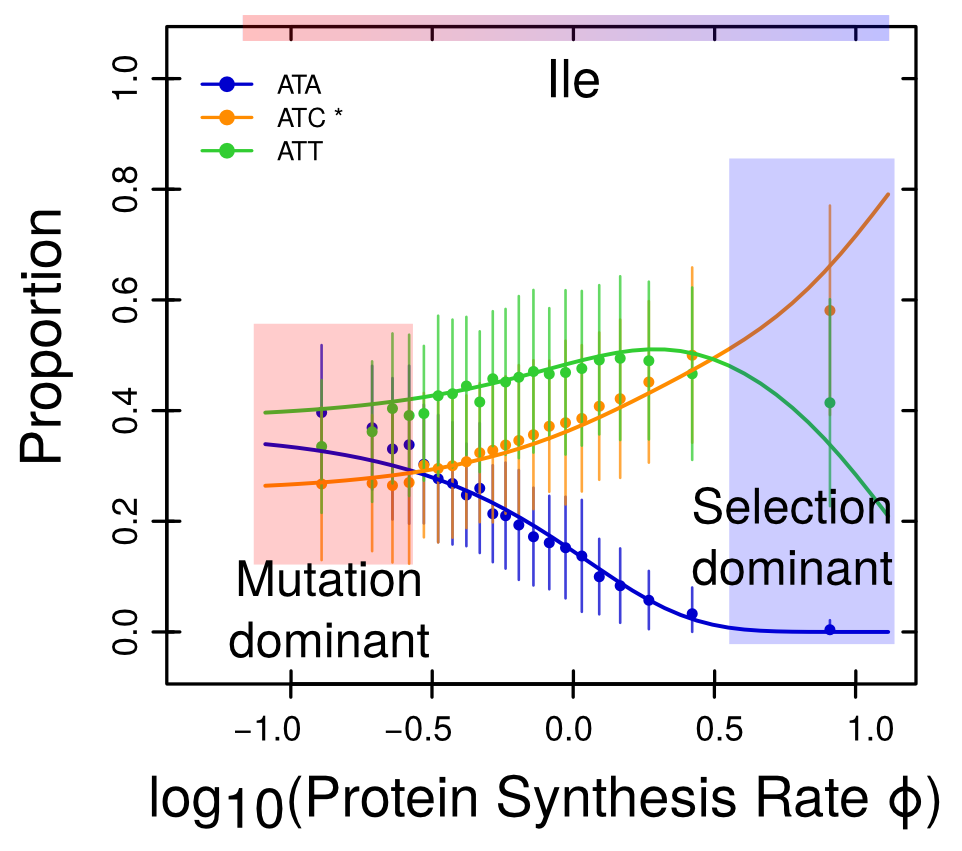
\includegraphics[width=0.6\textwidth]{ch1/expl_model}
	\caption{\ROC model behavior for Isoleucine.
	The proportion of each codon observed changes with protein synthesis rate.
	Mutation is dominant when protein synthesis rate is low, mutationally favored codons are observed with the highest frequency.
	With the increase of protein synthesis rate, the influence of selection increases until the system is dominated by selection.
	The selectively favored codon is observed with the highest frequency.}
	\label{fig:expl_model}
\end{figure}
\doublespacing

For example, strand specific mutation bias \citep{Lafay1999,Romero2000}, differences in the tRNA pool throughout life stages \citep{sagi2016}, or introgressions and horizontal gene transfer \citep{medigue1991,lawrence1997} can produce multiple genomic environments.
Chapter \ref{ch:anacoda} extends the mechanistic model \ROC \cite{gilchrist2015} to allow for a mixture distribution of mutation and selection parameters \cite{landerer2018} and provides researchers with a software tool to address intra genomic variation in codon usage.
However, there is a significant difference to classical mixture approaches.
In addition to gene population specific parameters, \ROC also estimates a gene specific parameter (protein synthesis rate). 
Therefore, the protein synthesis rate for each gene has to be estimated assuming that the a gene is in each gene population.
This can provide additional insight into the adaptiveness of a gene to alternative genomic environments.
Figure \ref{fig:expl_model} illustrates how the proportions of synonymous codons change with increasing protein synthesis rate.
When the protein synthesis rate is low, mutation bias between codons dominates the proportions of synonymous codons while increasing protein synthesis increases the strength of selection (see \cite{gilchrist2015} for details). 

In chapter \ref{ch:kluyveri}, I apply AnaCoDa to analyze the synonymous codon usage of the yeast \kluyveri which experienced a large scale introgression replacing the whole left arm of chromosome C \citep{friedrich2015}.
I studied the differences in the parameters describing codon usage between the endogenous \kluyveri genes and the introgressed exogenous genes.
Recognizing the differences in codon usage between the endogenous and exogenous genes allowed me to improve prediction of protein synthesis rate, and separate the effects of mutation bias and selection in the endogenous \kluyveri genes and the introgressed exogenous genes.
This information was used to determine a potential donor lineage in \gossypii, estimate the time since introgression, and estimate the genetic load of the introgression.

\section{Benefit: Selection on Amino acids}
Genes are evolving with natural selection favoring proteins that encode their function optimally, with mutations and genetic drift reducing functionality.
Amino acid preference and the relative strength of mutation, selection, and genetic drift usually varies between sites along the protein sequence.
The number of parameters required to describe protein fitness increases exponentially with the length of the protein if interactions between sites are accounted for.
Attempts to incorporate selection into phylogenetic approaches are, therefore, limited to site specific selection.
The goal of chapter \ref{ch:phylogeny} is to estimate the strength of site specific selection on amino acids from protein coding sequences in a phylogenetic framework.

\singlespacing
\begin{figure}
     \centering
	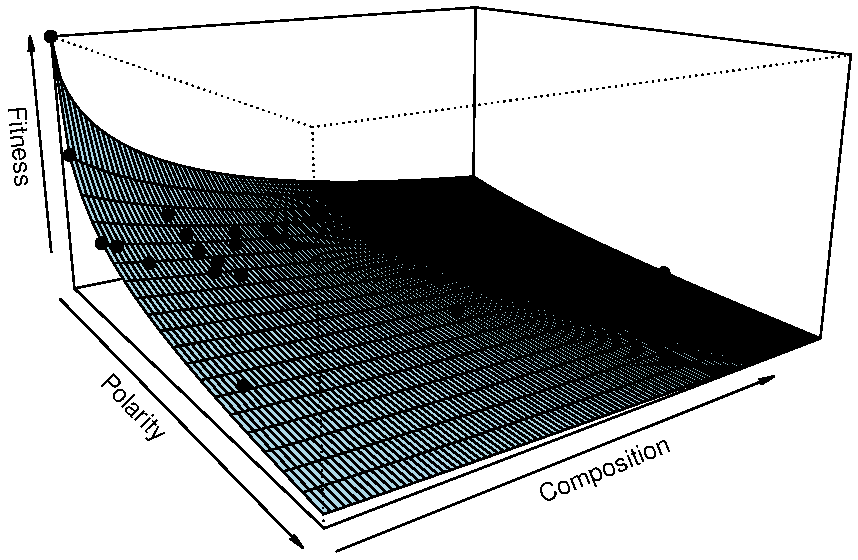
\includegraphics[width=0.7\textwidth]{ch1/decl_fitness2}
	\caption{Decline in fitness with distance in \PC space from the optimal amino acid. 
	Fitness decline of amino acids (black dots) relative to optimal amino acid (Alanine). Weighting of \PC properties according to \citet{grantham1974}.
	The full fitness surface can be described but only 20 discrete amino acid states are available for selection to act on.}
	\label{fig:decl_fit}
\end{figure}
\doublespacing

Ignoring interactions between sites allows to describe the site specific fitness landscape of a protein.
Some approaches rely on the description of the full fitness landscape and therefore require $19 \times L$, where $L$ is the length of the peptide in amino acids, parameters \citep{LartillotAndPhilippe2004,le2008,wang2008,holder2008,wu2013,tamuri2014}.
As this is still a large number of parameters the incorporation of experimentally determined site specific selection on amino acids is an attractive alternative \citep{bloom2014, thyagarajan2014, bloom2017}. 
Alternatively, assumptions about the nature of selection can reduce the number of parameters required.
For example, negative frequency dependent selection \citep{GoldmanAndYang1994, MuseAndGaut1994, thorne1996} or stabilizing selection \citep{beaulieu2019} allow for a reduction in fitness of amino acids with distance in \PC space.

\selac \citep{beaulieu2019}, a model of stabilizing selection, assesses the fitness of each amino acid relative to the fitness peak (Figure \ref{fig:decl_fit}).
Fitness is assumed to decline exponentially with distance in \PC space to the optimal amino acid.
In chapter \ref{ch:phylogeny} I apply \selac to the $\beta$-lactamase TEM and estimate site specific selection on amino acids and compare the inferred fitness landscape to empirical estimates from deep mutation scanning experiments \citep{stiffler2016}.
I find that experimentally informed amino acid preferences improve model fit but do not accurately reflect the evolution of TEM.
Furthermore, I show that the information on site specific selection on amino acids can be extracted from protein coding sequences by models rooted in first principles like \selac.




